\section{Sharding.}

MongoDB utiliza esta técnica para gestionar la carga de los servidores. Distribuye los datos entre distintos shards (conjuntos de servidores que almacenan parte de los datos), para que la carga a la hora de realizar consultas e inserciones se reparta.

\subsection{Pasos para la generación de resultados:}

Levantamos cinco shards siguiendo las instrucciones del archivo tutorial\_sharding.txt.

Luego creamos un indice simple sobre el atributo codigo\_postal.

Luego importamos el código de insert\_data.js donde tenemos
funciones que nos permiten ingresar datos de a 20k y pedir las estadísticas.
Finalmente, nos guardamos las estadísticas en archivos .txt. Los mismos se encuentran en
la carpeta mediciones.

\textbf{Generacion de Datos (insert\_data.js)}
\begin{lstlisting}
var insertData = function(dbName, colName, num) 
{
	var col = db.getSiblingDB(dbName).getCollection(colName);
	
	for (i = 0; i < num; i++) 
	{
		x = Math.floor(Math.random() * 1000000);
		doc = 
		{
			nombre: 'Martin Juarez',
			password: 'asdasd' ,
			codigo_postal: x,
			genero: 'masculino',
			edad: 29,
			fecha_creacion: '30/02/2015'
		}
		col.insert(doc);
	}
	
	print(col.count());
	print(col.getShardDistribution());
	print("##############################################");
}

var insertDataTotal = function(dbName, colName, step, total) 
{
	var col = db.getSiblingDB(dbName).getCollection(colName);
	
	while(col.count() < total)
	{
		for (i = 0; i < step; i++) 
		{
			x = Math.floor(Math.random() * 1000000);
			doc = {
				nombre: 'Martin Juarez',
				password: 'asdasd' ,
				codigo_postal: x,
				genero: 'masculino',
				edad: 29,
				fecha_creacion: '30/02/2015'
			}
			col.insert(doc);
		}
		
		print(col.count());
		print(col.getShardDistribution());
		print("##########################################");
	}
}
\end{lstlisting}
\subsection{Resultados}
\begin{figure}[H]
\centering
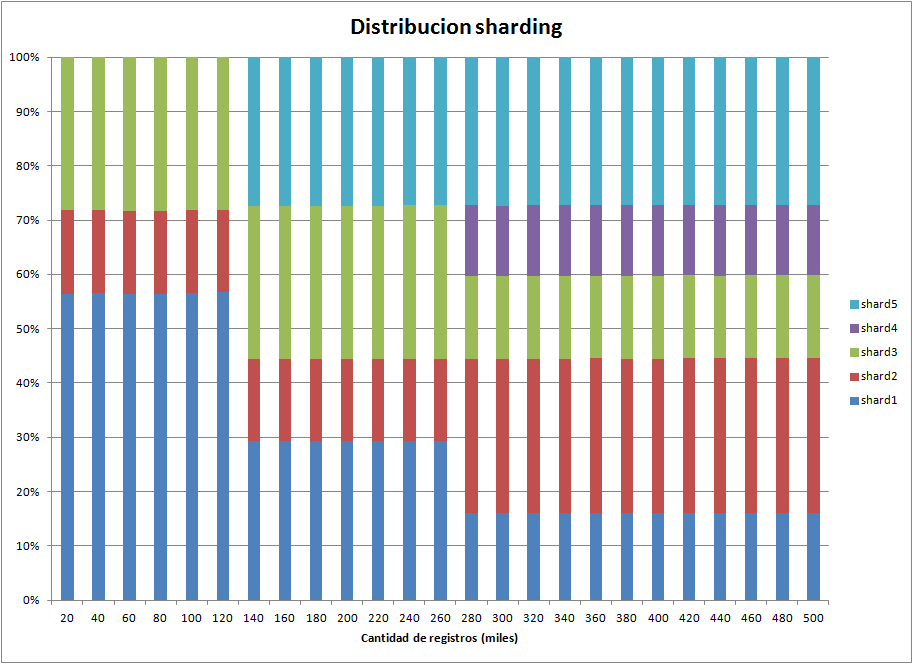
\includegraphics[width=165mm]{../mediciones/sharding_simple.png}
\caption{Porcentaje de distribucion entre los shards usando un
indice simple en base al codigo postal.}
\end{figure}
El primer resultado obtenido corresponde a la distribución de carga con el indice simple sobre código postal. En este caso la distribución no es uniforme, al comienzo gran parte de la carga se la lleva el Shard1 y no intervienen los Shard4 y Shard5. Esto es asi, porque se van llenando los primeros Shards, cuando esto ocurre luego de insertar unos 140.000 registros, vemos que comienzan a distribuirse en el Shard5, y el peso del Shard1 baja a un 30\%.
Al insertar unos 280.000 registros, y de ahí en adelante, el Shard4 comienza a registrar carga. Y en general, todos los shards tienen documentos. 

Ahora veremos como influye la generación de un indice Hash en base al \_id.
\begin{figure}[H]
\centering
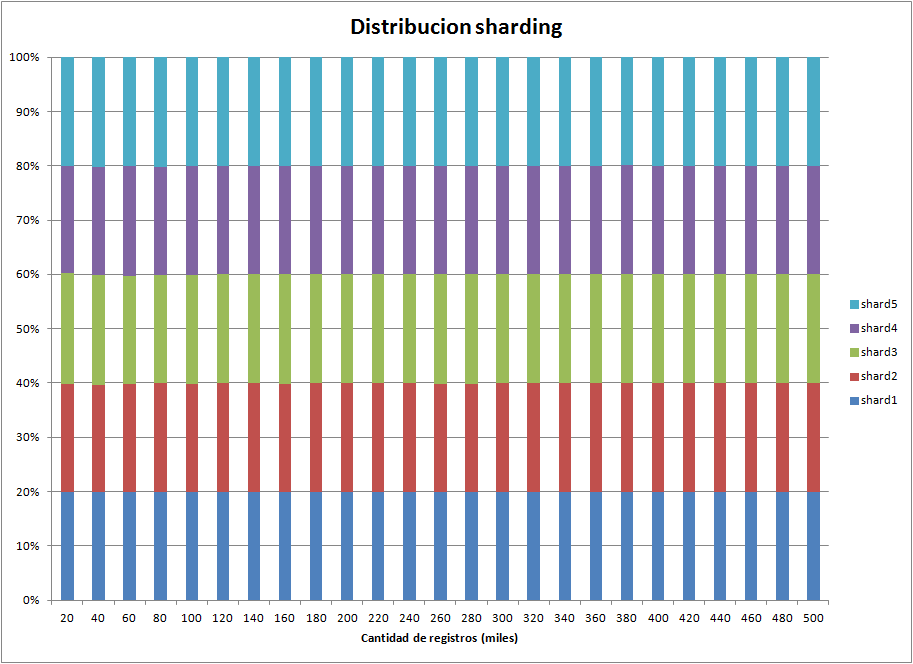
\includegraphics[width=165mm]{../mediciones/sharding_hashed.png}
\caption{Porcentaje de distribución entre los shards usando un
indice hasheado en base al \_id}
\end{figure}

En este caso, el indice hash hace que la distribución de los documentos sea muy equitativa entre los distintos Shards. Desde el comienzo de la carga de registros, se puede ver que todos los Shards tienen aproximadamente un 20 \% de carga.

Esto nos hace reflexionar sobre la importancia de la elección de los indices y su influencia en la distribución de la carga.

Los atributos deben poseer ciertas características para ser candidatos a claves en un esquema de Sharding. La distribución de sus valores debe ser lo mas equiprobable posible dentro de los distintos Shards. Por ejemplo, si tomamos Edad como clave en modelo de pirámide poblacional de un país, es probable que la distribución este mas concentrada en algunos Shards y no en otros. Los shards que contengas las edades mayores a 60 o 70 años tendrán pocos documentos. Dependiendo el país que tomemos, encontraremos mayor distribución de documentos en edades medias o en edades menores a 20 años.

Lo importante es encontrar claves dentro del modelo que reflejen una distribución equiprobable(o similar) y con esto, garantizar un balance de carga entre los diferentes Shards.



